\newcommand{\sor}[0]{\texttt{so }} 
\newcommand{\visib}[0]{\texttt{vis }} 
%\newcommand{\tool}[0]{\textsc{syncope}} % short for SYNthesizing

\documentclass[authorversion]{sig-alternate-05-2015}
%\usepackage[a4paper]{geometry}
\usepackage[utf8]{inputenc}
\usepackage{lipsum}
\usepackage{etoolbox}
\usepackage{makeidx}  % allows for indexgeneration
\usepackage{xspace}
\usepackage{comment}
\usepackage{mathpartir}
\usepackage{wrapfig}
\usepackage[inline]{enumitem}
\usepackage{bussproofs}
\usepackage{bussproofs}
\usepackage{dsfont}
\usepackage{xspace}
\usepackage{mathtools}
\usepackage{mathpartir}
\usepackage{listings}
\usepackage{color}
\usepackage{pifont}
\usepackage{amssymb}
\usepackage{moresize}
\usepackage[T1]{fontenc}
\usepackage[utf8]{inputenc}
\usepackage{sidecap}
\usepackage{framed}
\usepackage{subfigure}
\makeatletter
\patchcmd{\maketitle}{\@copyrightspace}{}{}{}
\makeatother
\usepackage[british]{babel}

\begin{document}

\newcommand{\tool}[0]{{\sc syncope}} % short for SYNthesizing
% COnsistency Property Enforcement.
\newcommand{\conj}{~\wedge~}

\newcommand{\HA}{{\sf HA}}
\newcommand{\SA}{{\sf SA}}
\newcommand{\UA}{{\sf UA}}
\newcommand{\scc}{\psi_{\sf sc}}
\newcommand{\ccc}{\psi_{\sf cc}}
\newcommand{\ecc}{\psi_{\sf ec}}
\newcommand{\rcc}{\psi_{\sf rc}}
\newcommand{\mavc}{\psi_{\sf mav}}
\newcommand{\rrc}{\psi_{\sf rr}}
%\newcommand{\coloneqq}{::=}
\newcommand{\spc}{\quad}





%=====================================================
%===============     SYNCOPE     =====================
%=====================================================
% data objects
\newcommand{\xO}{\N{\texttt{x}}}
\newcommand{\yO}{\N{\texttt{y}}}
% replicas
\newcommand{\replO}[1] {\N{\texttt{\#\vspace{0.55mm}}}#1}
% state values
\newcommand{\vO}{\N{\texttt{v}}}
% oprtations
\newcommand{\opO}{\N{\texttt{op}}}

% the relations relating effects in the store
\newcommand{\visO}{\N{\texttt{vis}}}
\newcommand{\soO}{\N{\texttt{so}}}

%types of contracts
\newcommand{\LB}{{\footnotesize$\textsf{LB}$}}
\newcommand{\UB}{{\footnotesize$\textsf{UB}$}}


%self contained sets of effects
\newcommand{\SC}[3] {\N{\mathbb{SC}}^{#1}_{#2}\vspace{0.55mm}(#3)}

% degree of dependency
\newcommand{\DDP}{{\footnotesize$\textsc{DDP}$}}

% bank account operations
\newcommand{\dRV}{{\footnotesize$\texttt{deposit}$}}
\newcommand{\wdRV}{{\footnotesize$\texttt{withdraw}$}}
\newcommand{\gbRV}{{\footnotesize$\texttt{get\_balance}$}}

% contracts
\newcommand{\rmwCTRT}{{\footnotesize$\textsc{RMW}$}}
\newcommand{\visCTRT}{{\footnotesize$\textsc{2VIS}$}}
\newcommand{\mwCTRT}{{\footnotesize$\textsc{MW}$}}
\newcommand{\mrCTRT}{{\footnotesize$\textsc{MR}$}}




%=====================================================








% \newtheorem{theorem}{Theorem}
% \newtheorem{lemma}[theorem]{Lemma}
% \newtheorem{proposition}[theorem]{Proposition}
% \newtheorem{corollary}[theorem]{Corollary}
% \newtheorem{definition}[theorem]{Definition}
% \newcounter{hno}
%   \newcounter{gno}
% \renewenvironment{proof}{\setcounter{hno}{0}\setcounter{gno}{0}
%   \emph{Proof.}}{}
% \newcommand{\npp}{\thehno \stepcounter{hno}}
% \newcommand{\mpp}{\thegno \stepcounter{gno}}

% ------- the application example commands
\newcommand{\stateC}{$\mathtt{State}$}
\newcommand{\effectC}{$\mathtt{Effect}$}
\newcommand{\writeC}{$\mathtt{write}$}
\newcommand{\readC}{$\mathtt{read}$}
\newcommand{\applyC}{$\mathtt{apply}$}

\newcommand{\seedS}{$\mathtt{rel. seed}$}
\newcommand{\propS}{$\mathtt{prop}$}
\newcommand{\relationS} {$\mathtt{relation}$}
\newcommand{\specS}{$\mathtt{spec}$}

\newcommand{\nullR}{\mathtt{null}}


\newcommand{\nonvisrule}{\rulelabel{non-vis exec}\hspace{0.67mm}}
\newcommand{\visrule}{\rulelabel{vis exec}\hspace{0.67mm}}

\newcommand{\stretcharraybig}{\renewcommand*{\arraystretch}{1.25}}
\newcommand{\cureff}{\hat{\eta}}
\newcommand{\eff}{\eta}
\newcommand{\fresh}{\N{\sf fresh}}
\newcommand{\cv}{\psi}
\newcommand{\ALT}{~\mid~}
\newcommand{\eid}{{\iota}}
\newcommand{\ObjType}{{\sf ObjType}}
\newcommand{\AbsType}{{\sf AbsType}}
\newcommand{\dom}{{\sf dom}}
\newcommand{\DtLib}[1]{\mathbb{D}(#1)}
\newcommand{\DtLibZ}{\mathbb{D}}
\newcommand{\Ops}{\Lambda}
\newcommand{\Ctrts}{\Psi}
\newcommand{\true}{\N{\textsf{true}}}

\newcommand{\R}[1]{\textrm{#1}}
\newcommand{\N}[1]{{\normalfont #1}}
\newcommand{\ObjZ}{\N{\textsf{Obj}}}
\newcommand{\Obj}[1]{\N{\textsf{Obj}_{#1}}}
\newcommand{\ReplID}{\mathtt{ReplID}}
\newcommand{\SessID}{\mathtt{SessID}}
\newcommand{\typeFun}[1]{\N{\textsf{type}}(#1)}
\newcommand{\Op}[1]{\N{\textsf{Op}_{#1}}}
\newcommand{\set}[1]{\mathcal{P}(#1)}
\newcommand{\unitVal}{\N{\textsf{unit}}}
\newcommand{\EffUniv}{\N{\sf Effect}}
\newcommand{\EffID}{\mathtt{SeqNo}}
\newcommand{\TransID}{\N{\sf TransID}}
\newcommand{\AVal}[1]{\N{\textsf{AVal}_{#1}}}
\newcommand{\RVal}[1]{\N{\textsf{RVal}_{#1}}}
\newcommand{\Eff}[1]{\N{\textsf{Eff}_{#1}}}
\newcommand{\loud}[1]{\textbf{\textit{#1}}}
\newcommand{\dt}[1]{\mathcal{D}_{#1}}
\newcommand{\vis}[2]{\N{\textsf{vis}(#1,#2)}}
\newcommand{\visZ}{\N{\textsf{vis}}}
\newcommand{\depsZ}{\N{\textsf{deps}}}
\newcommand{\deps}[1]{\N{\textsf{deps}(#1)}}
\newcommand{\Rvis}{\N{\textsf{vis}}}
\newcommand{\arZ}{\N{\textsf{ar}}}
\newcommand{\ar}[2]{\N{\textsf{ar}(#1,#2)}}
\newcommand{\stxZ}{\sim}
\newcommand{\stx}[2]{#1\sim#2}
\newcommand{\nstx}[2]{#1\not\sim#2}
\newcommand{\comZ}{\N{\textsf{com}}}
\newcommand{\com}[1]{\comZ(#1)}
\newcommand{\so}[2]{\N{\textsf{so}(#1,#2)}}
\newcommand{\soZ}{{\textsf{so}}}
\newcommand{\stZ}{\N{\textsf{st}}}
\newcommand{\Rso}{\N{\textsf{so}}}
\newcommand{\Rst}{\N{\textsf{st}}}
\newcommand{\COM}{\textrm{\sc {\small Commit}}}
\newcommand{\soo}[2]{\N{\textsf{soo}(#1,#2)}}
\newcommand{\sooZ}{\N{\textsf{soo}}}
\newcommand{\hb}[2]{\N{\textsf{hb}(#1,#2)}}
\newcommand{\hbo}[2]{\N{\textsf{hbo}(#1,#2)}}
\newcommand{\hbZ}{\N{\textsf{hb}}}
\newcommand{\hboZ}{\N{\textsf{hbo}}}
\newcommand{\txnZ}{\N{\textsf{txn}}}
\newcommand{\txn}[2]{\txnZ\{#1\}\{#2\}}
\newcommand{\trunc}[1] {\N{\textsf{trunc\vspace{0.55mm}}}(#1)}
\newcommand{\sameobj}[2]{\N{\textsf{sameobj}(#1,#2)}}
\newcommand{\sameobjZ}{\N{\textsf{sameobj}}}
\newcommand{\sametxn}[2]{\N{\textsf{sametxn}(#1,#2)}}
\newcommand{\sametxnZ}{\N{\textsf{sametxn}}}
\newcommand{\E}{\N{\textsf{E}}}
\newcommand{\Pool}{\N{\textsf{pool}}}
\newcommand{\Cache}{\N{\textsf{cache}}}
\newcommand{\Avail}{\N{\textsf{DDP}}}
\newcommand{\CacheFinder}{\N{\textsf{Ctxt}}}
\newcommand{\EffSoup}{\N{\textsf{A}}}
\newcommand{\myif}{\mathtt {if}}
\newcommand{\rel}{\mathtt{r}}
\newcommand{\V}{\N{\textsf{V}}}
\newcommand{\Set}{\N{\textsf{S}}}
\newcommand{\Rel}{\N{\textsf{R}}}
\newcommand{\op}{\N{\textsf{op}}}
\newcommand{\obj}{\N{\textsf{obj}}}
\newcommand{\dep}{\N{\textsf{dep}}}
\newcommand{\ssn}{\N{\textsf{ssn}}}
\newcommand{\id}{\N{\textsf{id}}}
\newcommand{\oper}{\N{\textsf{oper}}}
\newcommand{\rval}{\N{\textsf{rval}}}
\newcommand{\repl}{\N{\textsf{repl}}}
\newcommand{\sess}{\N{\textsf{sess}}}
\newcommand{\rdtspec}{\Delta}
\newcommand{\goesto}{\longrightarrow}
\newcommand{\tuplee}[1]{\langle #1 \rangle}
\newcommand{\ctxtFn}{\N{\textsf{ctxt}}}
\newcommand{\rdtredsto}{\N{\leadsto}}
\newcommand{\Exec}{\N{\textsf{(\EffSoup,\allowbreak \visZ,\allowbreak \soZ)}}}
\newcommand{\pll}{~\|~}
\newcommand{\Mod}[1]{\N{\textsf{Mod}}(#1)}
\newcommand{\De}[1]{#1}
\newcommand{\Der}[2]{[\![#1,#2]\!]_{r}}
\newcommand{\msentails}[2]{#1 \models #2}
\newcommand{\hasTyp}[2]{#1 \vdash #2}
\newcommand{\auxred}[4]{#1 \vdash #2 \xhookrightarrow{#3} #4 }
\renewcommand{\qed}{\nobreak \ifvmode \relax \else
      \ifdim\lastskip<1.5em \hskip-\lastskip
      \hskip1.5em plus0em minus0.5em \fi \nobreak
      \vrule height0.75em width0.5em depth0.25em\fi}


% Operational semantics rules
\newcommand{\rulelabel}[1]{\textrm{\sc {\small \scriptsize [#1]}}}
\newcommand{\RULE}[3]
{\frac{\begin{array}{c}#1\end{array}}
		 {\begin{array}{c}#2\end{array}}
~ \rulelabel{#3}
}

\newcommand{\RuleTwo}[2]
{\frac{\begin{array}{c}#1\end{array}}
		 {\begin{array}{c}#2\end{array}}
}

\newenvironment{nop}{}{}
\newenvironment{smathpar}{
\begin{nop}\small\begin{mathpar}}{
\end{mathpar}\end{nop}\ignorespacesafterend}
\newenvironment{fmathpar}{
\begin{nop}\scriptsize \begin{mathpar}}{
\end{mathpar}\end{nop}\ignorespacesafterend}


\newenvironment{cmathpar}{
\vspace{-3mm}
\renewcommand{\arraystretch}{1.2}
\begin{nop}\begin{mathpar}}{
\end{mathpar}\end{nop}\ignorespacesafterend}

\newcommand{\rsf}[1]{\R{\sf #1}}
\newcommand{\trans}[4]{\N{\textsf{trans}}\{#1,#2\}\{#3,#4\}}

\setlength{\floatsep}{5pt}
\setlength{\textfloatsep}{10pt}
\setlength{\dblfloatsep}{5pt}
\setlength{\dbltextfloatsep}{10pt}


\newcommand{\ecds}{ECDS\xspace}
%\newcommand{\nexists}{\not\exists}
%\newcommand{\nsucc}{\not\succ}
%\newcommand{\nsubseteq}{\not\subseteq}



% Copyright

%\CopyrightYear{2018} 
%\setcopyright{acmcopyright}
%\conferenceinfo{PaPOC'8,}{April 18-21, 2016, London, United Kingdom}
%\isbn{978-1-4503-4296-4/16/04}\acmPrice{\$15.00}
%\doi{http://dx.doi.org/10.1145/2911151.2911160}


\title{Fine-grained Distributed Consistency Guarantees with Effect
Orchestration}
%
% You need the command \numberofauthors to handle the 'placement
% and alignment' of the authors beneath the title.
%
% For aesthetic reasons, we recommend 'three authors at a time'
% i.e. three 'name/affiliation blocks' be placed beneath the title.
%
% NOTE: You are NOT restricted in how many 'rows' of
% "name/affiliations" may appear. We just ask that you restrict
% the number of 'columns' to three.
%
% Because of the available 'opening page real-estate'
% we ask you to refrain from putting more than six authors
% (two rows with three columns) beneath the article title.
% More than six makes the first-page appear very cluttered indeed.
%
% Use the \alignauthor commands to handle the names
% and affiliations for an 'aesthetic maximum' of six authors.
% Add names, affiliations, addresses for
% the seventh etc. author(s) as the argument for the
% \additionalauthors command.
% These 'additional authors' will be output/set for you
% without further effort on your part as the last section in
% the body of your article BEFORE References or any Appendices.

\numberofauthors{3} %  in this sample file, there are a *total*
% of EIGHT authors. SIX appear on the 'first-page' (for formatting
% reasons) and the remaining two appear in the \additionalauthors section.
%
\author{
% You can go ahead and credit any number of authors here,
% e.g. one 'row of three' or two rows (consisting of one row of three
% and a second row of one, two or three).
%
% The command \alignauthor (no curly braces needed) should
% precede each author name, affiliation/snail-mail address and
% e-mail address. Additionally, tag each line of
% affiliation/address with \affaddr, and tag the
% e-mail address with \email.
%
% 1st. author
\alignauthor
Kia Rahmani \\ 
       \affaddr{Purdue University}\\
       \affaddr{USA}\\
       \email{rahmank@purdue.edu}
% 2nd. author
\and \alignauthor
Gowtham Kaki\\ 
       \affaddr{Purdue University}\\
       \affaddr{USA}\\
       \email{gowtham@purdue.edu}
% 3rd. author
\and \alignauthor Suresh Jagannathan\\
       \affaddr{Purdue University}\\
       \affaddr{USA}\\
       \email{suresh@cs.purdue.edu}
}
% There's nothing stopping you putting the seventh, eighth, etc.
% author on the opening page (as the 'third row') but we ask,
% for aesthetic reasons that you place these 'additional authors'
% in the \additional authors block, viz.

% Just remember to make sure that the TOTAL number of authors
% is the number that will appear on the first page PLUS the
% number that will appear in the \additionalauthors section.

\maketitle


\begin{abstract}
\end{abstract}

\keywords{Runtime Safety; Weak Consistency; Key-value stores; Haskell}







%-----------------------
%-----------------------
%-----------------------
%-----------------------
%SECTION  1
\section{Introduction}

Historically, the \emph{de facto} system abstraction for developing distributed
programs has typically included ACID\footnote{Atomicity, Consistency,
Isolation and Durability} properties. These properties
guarantee replication transparency and make it
straightforward to develop standardized implementation and reasoning
techniques around \emph{strongly consistent} (SC) distributed stores \cite{papa,lin}.
However, for web-scale applications that need to be “always-on” even
in the presence of network partitions, extensive
synchronization overhead is often unacceptable \cite{cap}.
Such applications are therefore usually designed to tolerate certain
inconsistencies, allowing them to adopt weaker notions of consistency
that impose less synchronization overhead such as \emph{eventual
consistency} (EC). 

Applications that may not tolerate the level of inconsistency imposed by EC 
are often equipped with ad-hoc mechanisms to prevent 
undesirable anomalies allowed in EC stores, where the local state of
each application server only represents an \emph{unspecified order} of an
\emph{unspecified subset} of the aggregate collection of all updates
submitted to the system globally. Unfortunately, such enforcement
mechanisms are closely tied to the application logic, confounding
standardization, while complicating application reasoning,
maintainability, and reusability.

In this paper, we propose an alternative approach to weak consistency
enforcement that circumvents the aforementioned issues. \tool\; is a
lightweight runtime verification system for Haskell that allows
application developers to take advantage of weak consistency without
having to re-engineer their code to accommodate anomaly preemption
mechanisms by declaratively admitting consistency
requirements via a specification language.

The remainder of this paper is organized as follows:
Section 2 introduces our system model and in Section 3 we 
discuss different approaches on distributed consistency enforcement which we
collectively refer to as \emph{orchestration} techniques. In sections 4 and 5 we present
evidence for real-world applications requiring fine-grained consistency guarantees and 
experimental results suggesting the possiblility of performance gain in off-the-shelf datastores deploying fine-grain consistency guarantees using out tool. 
We present our conclusions and a review of the related works in section 8.
%---------------------------------------------------------------------------------------------------------------



%-----------------------
%-----------------------
%-----------------------
%-----------------------
%SECTION 2
\section{System Model}
A data store in our system model is a collection of replicas (\#1,\#2,...), each of
which maintains a copy of a set of replicated data object ($x$,$y$,...). 
Each data object includes and maintains a state value ($v$,$v'$,...) and is equipped with a set of 
operations ($op$,$op'$,...). Operations may read the state of an object residing 
in a replica, and modify it by generating update \emph{effects} ($\eta$,$\eta'$,...). 
These effects are then {\bf asynchronously} sent to all other replicas where they are applied to the state 
of the object instance at the recipient replica. 
Fig.~1(a) and Fig.~1(b) illustrate this process.


%-----------------------
%The system model figure
\begin{figure}[h]
	\subfigure[{\small A client operation is routed to replica \#1.}]{\label{fig:sys_a}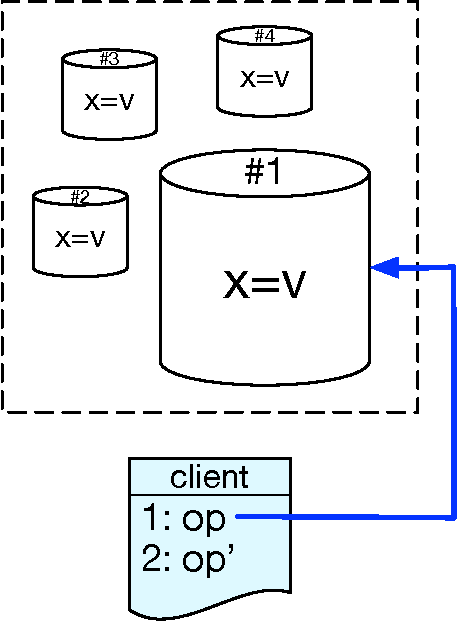
\includegraphics[scale=0.27]{Figures/system_model1.pdf}}
	\hfill \vline \hfill
	\subfigure[{\small An effect is created and propagated}]{\label{fig:sys_b}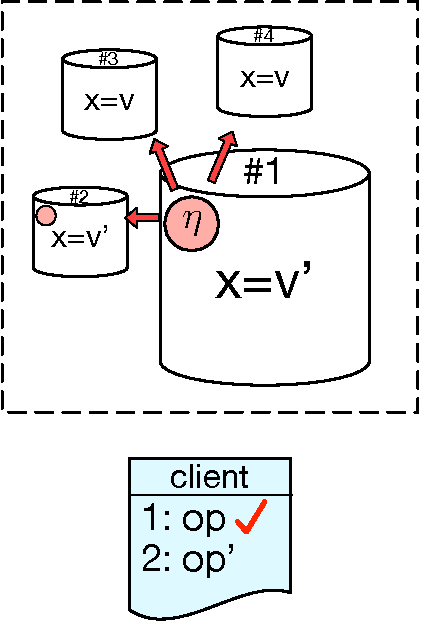
\includegraphics[scale=0.27]{Figures/system_model2.pdf}}
	\hfill \vline \hfill
	\subfigure[{\small Second operation is routed to the replica \#4}]{\label{fig:sys_c}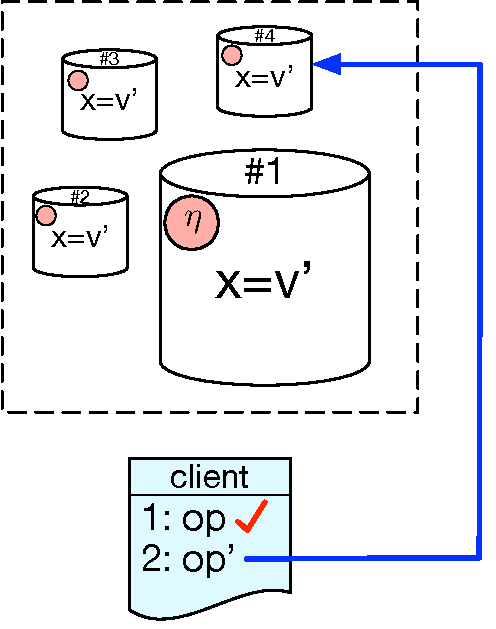
\includegraphics[scale=0.27]{Figures/system_model3.pdf}}
\label{fig:sys}
\caption{System Model}
\end{figure}
%-----------------------
%
In order to admit all inconsistencies and anomalies associated with EC we assume no direct synchronization between replicas when an operation is 
executed and as a result, concurrent and possibly conflicting updates can be generated
at different replicas.
Conflict resolution is handled at the point when an effect is applied to the 
current state of the object, and must be designed to ensure that all replicas 
eventually converge to the same value. 

Clients in our model interact with the store by invoking operations on objects. 
A \emph{session} is a sequence of operations invoked by a particular client. 
Consequently, operations (and effects) can be uniquely identified by their session id and 
their sequence number in that particular session, which is used by
replicas to record the set of all updates that are locally applied. 
Due to traffic balancing requirements, 
operations (even from the same session) might be routed to different replicas (Fig.~1(a) and Fig.~1(c)).

Lastly, we define two relations over effects. 
Session order (\sor) is an irreflexive, transitive relation that relates an effect
 to all subsequent effects from the same session. Visibility (\visib) is an 
irreflexive and assymetric relation that relates an effect to all others that are influenced 
by it (i.e., witnesses its update) at the time of their generation. 
For example, in Fig.\ref{fig:sys_c} \visib($\eta$,$\eta'$) holds, since $\eta$ (the effect of op) 
has already been delivered and applied to the replica \#4, when op' is 
executed and thus has influenced generation of $\eta$'.
%---------------------------------------------------------------------------------------------------------------


















%-----------------------
%-----------------------
%-----------------------
%-----------------------
%SECTION 3
\section{Effect Orchestration}
In this section we introduce \tool, a shim-layer for off-the-shelf EC key-value stores, 
which extends the basic consistency guarantees offered by them into a vast set of 
fine-grained guarantees (Fig.~2).
\tool's design realizes two fundamental classes of run-time procedures on effects and operations, 
combination of which is necessary to enforce fine-grained consistency requirements in a message-passing distributed system (such as our system model). In the following subsections, we will explain these techniques in detail.
\begin{figure}[h]
\centering
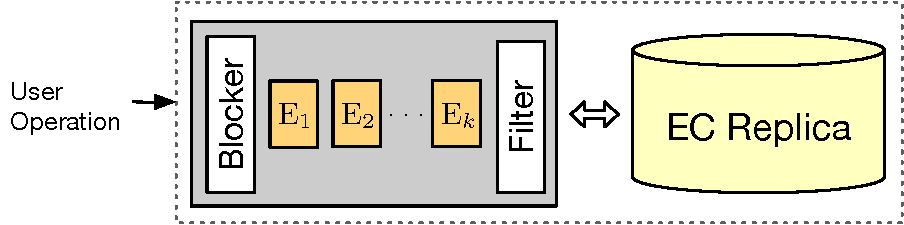
\includegraphics[scale=0.5]{Figures/shimlayer.pdf}
\label{fig:shim}
\caption{Shim Layer Layout}
\end{figure}

\subsection{Blocking}
\tool's first consistency enforcment technique is called \emph{blocking},
which is a generalized mechanism to stall a user operation until a certain set 
of \emph{necessary} dependencies of that operation become available at the underlying replica. 
\tool\; relies on the underlying store for effect propagation which guarantees the eventual delivery of all 
effects to all replicas. Consequently, all user operations will eventually proceed in an unpartitioned 
network\footnote{Detailed and formal explaination of all mechanisms with formal proofs of 
liveness, correctness and optimality can be found the longer version of this paper \cite{syncope}}. 

A use case of this technique is when two operations from the same session are routed to different replicas.
This can \emph{sometimes} be problematic, e.g. when a user deposits some money into her bank account and then queries the 
balance. If the effect of the deposit is not available at the replica executing the query, 
she might think that the bank has stolen her money.
In this scenario the second operation should be blocked, 
until the effect of the deposit operation is delivered to the replica. 

The effects that an operation must wait for, are known as the dependency set of that operation. 
In the following parts we will introduce a formal language that allows users to define 
a rich set of fine-grained dependencies for each operation, in order to 
prevent undesired behaviors in their application.
%---------------------------------------------------------------------------------------------------------------

\subsection{Filtration}
Similar to other systems offering add-on consistency guarantees for EC
key-value stores, \tool's shim layer also maintains
a \emph{safe} environment in the memory by periodically (or on-demand)
reading from the underlying EC database and adding the effects to the
environment, only if the dependencies of them have already been added to
the environment. 
For example, \cite{bolton,quelea} enforce causal
consistency using similar shim layers, which maintain consistent caches
that are guaranteed to
contain a \emph{causal cut} of the global execution history at any
given point in time.

\tool\; generalizes this idea into a fine-grained filtration mechanism
which maintains \emph{multiple} safe environments ($E_1$, $E_2$,...),
each for the use of a specific operation. Users then can specify arbitrary
consistency guarantees in a
language that is seeded with \sor and \visib relations and define constraints 
on read operations that can be used to synthesize appropriate filtration  mechanisms.

For example, in a microbloging application where Bob tweets two
consecutive related
messages $B_1$ and $B_2$, Alice who is connected to a different replica, should not be
able to read Bob's second message without witnessing the first. 
Fig.~3 (left) shows this scenario on an unprotected EC system which
permits this undesired anomaly. The middle and right parts of the figure
however,
depict how a simple
filteration mechanism can prevents Alice from seeing Bob's second
message by allowing $B_2$ into the memory only after $B_1$ is also
available. Even though filteration imposes extra staleness on the
underlying database (e.g. in the middle part of Fig.3), it is very
effective in eliminating many anomalous behaviors of applications
running under EC.

\begin{figure}[h]
\centering
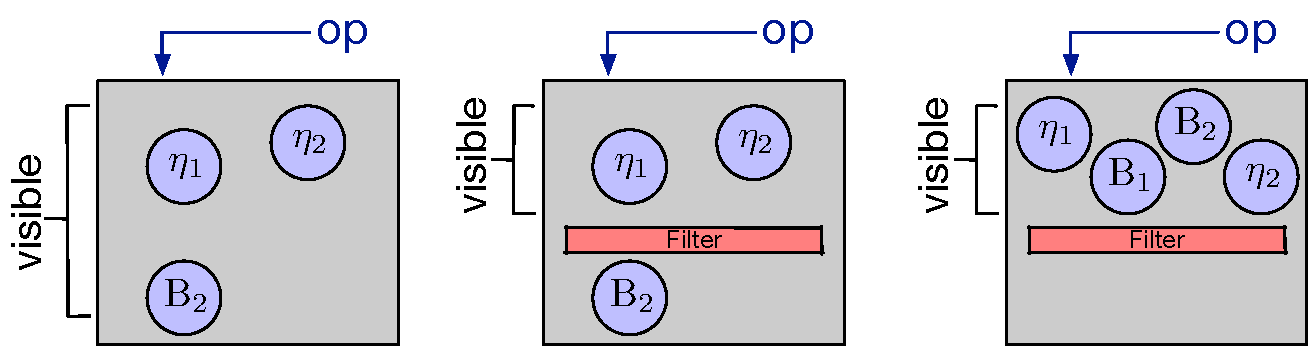
\includegraphics[scale=0.37]{Figures/ub.pdf}
\label{fig:filter}
\caption{Filteration}
\end{figure}
%---------------------------------------------------------------------------------------------------------------


\subsection{Specification Language}
The formal syntax of our specification (or contract) language, presented
in
Fig.~\ref{fig:ctrt_syntax}, allows definitiosn of
\propS{}, a first-order formula
that establishes dependency relations between effects,
necessary to determine the effects an operation may witness, under
a given consistency level.
\begin{figure}[h]
\centering
  \begin{fmathpar}
  \begin{array}{lclcl}
                \rel & \in & \texttt{rel.seed} & \coloneqq & \visZ \ALT
                \soZ \ALT \rel \cup \rel \\
               \Rel & \in & \texttt{relation} & \coloneqq &  \rel
               \ALT \Rel;\rel  \ALT \nullR  \\
             \pi & \in & \texttt{prop} & \coloneqq & \forall a.
      ~a \xrightarrow{R} \hat{\eff} ~\Rightarrow~ a \xrightarrow{\visZ}
      \hat{\eff}\\
                \psi & \in & \texttt{spec} & \coloneqq & \pi \ALT \pi \conj \pi
  \end{array}
  \end{fmathpar}
  \caption{Specification Language}
\label{fig:ctrt_syntax}
\end{figure}


The language is seeded with $\soZ$ and $\visZ$, respectively
representing session
order and visibility relations over effects,
and defines dependency \relationS{} as a sequence\footnote{\tool\; also
	allows
	using closures of seeds, which is omitted here for
simplicity.} of seeds,
where
({\footnotesize $a \xrightarrow{\rel_1;...;\rel_k} b$})
is interpreted as
{\footnotesize$\exists c. (a
	\xrightarrow{\rel_1;...;\rel_{k-1}} c
\wedge c \xrightarrow {\rel_k} b)$}.
$\nullR{}$ is the empty relation.
Additionally, the language allows conjunctions of propositions,
\specS{},
used to define a safe environment
free from \emph{multiple} inconsistencies.
Our language is crafted to capture all fine-grained weak consistency
levels, including well-known ones such as those explicated by Terry et
al. \cite{terry}
(see e.g., Fig.~\ref{fig:ctrt_example}).
\begin{figure}[h]
\centering
\begin{scriptsize}
\begin{tabular}{|l | c |}
\hline
 { \texttt Guarantee} & {\texttt Contract} \\ [0.5ex]
\hline
{\tiny \textsc{Read My Writes (RMW)}} & $\forall a. a ~  ~\xrightarrow{\soZ}  ~ ~
\hat{\eta} \Rightarrow a \xrightarrow{\visZ} \hat{\eta} $ \\
{\tiny \textsc{Monotonic Writes (MW)}} & $\forall a. a \xrightarrow{\soZ;\visZ}
\hat{\eta} \Rightarrow a \xrightarrow{\visZ} \hat{\eta} $ \\
{\tiny \textsc{Monotonic Reads (MR)}} & $\forall a. a \xrightarrow{\visZ;\soZ}
\hat{\eta} \Rightarrow a \xrightarrow{\visZ} \hat{\eta} $ \\
{\tiny \textsc{Transitive Visibility (2VIS)}} & $\forall a. a \xrightarrow{\visZ;\visZ}
\hat{\eta} \Rightarrow a \xrightarrow{\visZ} \hat{\eta} $ \\

\hline
\end{tabular}
\end{scriptsize}
\caption{Contract Examples}
\label{fig:ctrt_example}

\end{figure}

%---------------------------------------------------------------------------------------------------------------




















%-----------------------
%-----------------------
%-----------------------
%-----------------------
%SECTION 4
\section{Practicality}
In this section, we report on
benchmark applications that utilize fine-grained weak consistency
requirements, expressable
in \tool's specification language.
Fig.~\ref{fig:dist_table} presents seven such programs, that include
library definitions of individual replicated data types as well as
larger applications consisting of multiple replicated types.

Each program supports various operations, some of which have
non-trivial consistency requirements. Out of the 38 operations
defined in these programs, there are 11 such operations, whose
consistency requirements can be expressed as a combination of four
previously described consistency guarantees: Monotonic Reads (MR),
Monotonic Writes (MW), Read-My-Writes (RMW), and Transitive Visibility
(2VIS). The significant diversity among the consistency requirements
of these operations emphasizes the need for a multi-abled environment
that can understand and enforce fine-grained consistency requirements
efficiently. 
It is clearly not practical to hard code them all, due to
their sheer number; even if we ignore bespoke consistency
requirements, there are 15 combinations of just the 4 aforementioned
consistency guarantees. 

Causal
consistency (CC), the strongest of the weak consistency guarantees, is
often used as a metaphorical one-size to fit all weak consistency
requirements (including all the benchmarks above).  Notably, none of the operations we analyzed
intrinsically requires CC and the undesired anomalous behaviors could be prevented by combinations of weaker consistency levels, which \tool\; can enforce exactly as they are specified.
\begin{figure}[h]
\centering
\begin{center}
\begin{scriptsize}
\begin{tabular}{|l |  l | l|} 
\hline
 \multicolumn{1}{|c}  {\bf Benchmark} & \multicolumn{1}{c} {\bf
 Consistency} & \multicolumn{1}{c|}  {\bf
 Description}\\ [0.5ex] 
\hline
Counter  & MR & {\tiny
 \begin{tabular}[c]{@{}l@{}} Monotonicly increasing counter\\ e.g.
 YouTubes' watch count \end{tabular} 
 }\\ \hline
DynamoDB  & RMW & {
\tiny
 \begin{tabular}[c]{@{}l@{}} Integer register allowing\\ various
 conditional puts\\ and gets \end{tabular} 
} \\ \hline
Online Store & RMW &  {
\tiny
 \begin{tabular}[c]{@{}l@{}} Online store with shopping\\ carts
 and modifiable\\  item prices \end{tabular} 
} \\ \hline
Bankaccount  & 2VIS $\wedge$ RMW & {
\tiny
 \begin{tabular}[c]{@{}l@{}} Offering deposit, \\ withdraw and get \\ balance
 operations \end{tabular} 
}\\ \hline
Shopping List   &  MW $\wedge$ RMW & {
 \tiny
 \begin{tabular}[c]{@{}l@{}} A shopping list with \\ concurrent adds
	 and\\
 deletes \end{tabular} 
}\\ \hline 
Microblog  &  MW, RMW & {
 \tiny
 \begin{tabular}[c]{@{}l@{}} A Twitter-like application \\ modeled after
 Twissandra \cite{twis}\end{tabular} 
}\\\hline
Rubis  & RMW, RMW$\wedge$2VIS & {
 \tiny
 \begin{tabular}[c]{@{}l@{}} eBay-like application with \\ browsing,
 supporting user \\ wallet\end{tabular} 
} \\
\hline
\end{tabular}
\end{scriptsize}
\end{center}
\caption{Fine-grained consistency requirement in benchmark programs}
\label{fig:dist_table}
\end{figure}


\begin{comment}
\begin{figure}[b]
\centering
\begin{center}
\begin{scriptsize}
\begin{tabular}{|l |  l|}    
\hline
 \multicolumn{1}{|c}  {\bf Benchmark} & \multicolumn{1}{c|} {\bf
 Consistency} \\ [0.4ex]                           
\hline
Counter  & MR \\ \hline
DynamoDB  & RMW \\ \hline
Online Store & RMW \\ \hline
Bankaccount  & 2VIS $\wedge$ RMW \\ \hline
Shopping List   &  MW $\wedge$ RMW \\ \hline 
Microblog  &  MW, RMW \\\hline
Rubis  & RMW, RMW$\wedge$2VIS \\
\hline
\end{tabular}
\end{scriptsize}
\end{center}
\caption{Fine-grained consistency requirement in benchmark programs}
\label{fig:dist_table}
\end{figure}
\end{comment}





%---------------------------------------------------------------------------------------------------------------

















%-----------------------
%-----------------------
%-----------------------
%-----------------------
%5
\section{Evaluation}
\tool\; is implemented as an extension to a GHC Haskell add-on called
Quelea \cite{quelea}.  Quelea maintains a causally
consistent~\cite{bolton} cache on top of Cassandra, and \emph{all}
operations whose contract is satisfied under causal consistency, are
performed witnessing that cache (even if they require weaker
guarantees.).

In \tool, we maintain a generic cache in which operations maintained
by the cache are associated with tags, and are allowed to witnesses
only the subset of effects in the cache that also have that tag
(i.e. effects that are in the \emph{logical cache} associated with
that operation). We implemented a dependency finder mechanism in
\tool, that is used to verify the presence of arbitrarily defined
dependencies of an effect in each logical cache. Consequently, \tool's
filtration and blocking mechanisms are added to the runtime system,
which rely on this dependency finder to keep each logical cache
consistent according to its associated contract.

Considering the arbitrary length of the dependency relations that may
be generated and the fact that verifying the presence of dependencies for
an effect might fail for an unbounded number of trials until all
dependencies arrive, special care must be taken to ensure performance
does not grade at scale.  We implemented a number of techniques to
improve cache efficiency such as memoization that extends the binary
notion of dependency presence to the \emph{degree of dependency
  presence} (\DDP{}) representing the maximum \emph{depth} (or size)
of the dependencies of an effect, whose presence has already been
verified.  Consequently, when verification fails, we can avoid
checking previously computed and known dependencies when subsequent
effects arrive.  \tool's runtime, by performing periodic \DDP{}
refreshes, tries to assign larger \DDP{} values to each effect when
more dependencies arrive at the replica. The details of this
technique, captured as an operational semantics in available in the longer version of this paper 
\cite{syncope}.

\begin{figure*}[h]
\centering
	\subfigure[{\small Latency}]{\label{fig:latency}
\hfil

\includegraphics[scale=0.35]{Figures/latency.pdf}}
\hfil
	\subfigure[{\small Staleness}]{\label{fig:staleness}
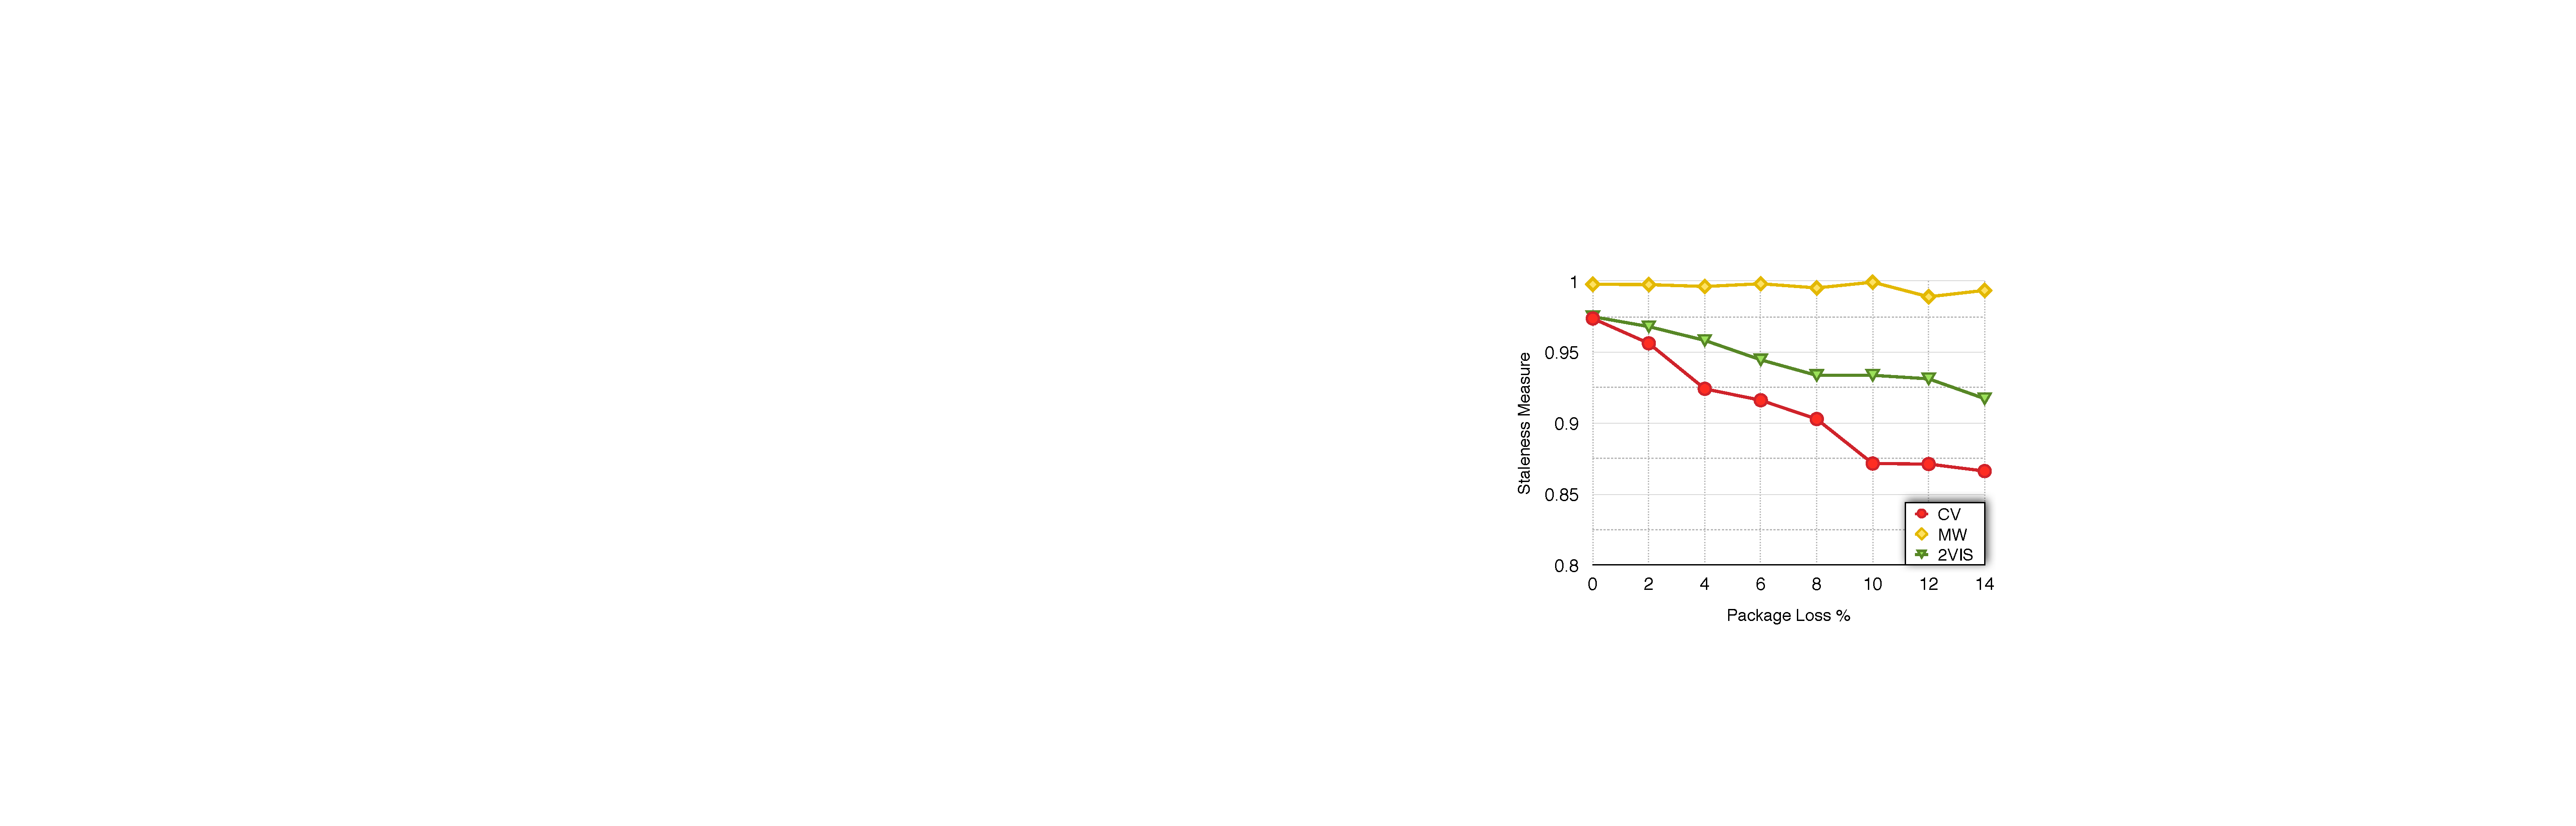
\includegraphics[scale=0.35]{Figures/staleness.pdf}}
\hfil
\label{fig:eval}
\caption{Performance Comparison}
\end{figure*}

We have deployed \tool\; on a cloud cluster,
consisting of three fully replicated Cassandra replicas, running on
separate machines within the same
datacenter.
Each machine is instantiated with a
\tool\; shim layer, that responds to clients,
 which are instantiated on a VM
co-located with one of the replicas on a machine.
We deploy the cluster on three \texttt{m4.4xlarge} Amazon EC2 instances
in the US-West (Oregon) region, with an inter-machine communication time of 5ms.

Inter-replica communication in Cassandra uses TCP connections, causing
all messages to get delivered with no loss and reordering, which is in
practice, far more consistent than EC, and masks out the performance
gain from our fine-grained consistency guarantees.  Consequently, to
simulate a realistic and pure EC environment, we injected artificial message
losses in \tool's shim layer, forcing random messages to be delayed
for 1s, simulating messages losses in a network with 600ms RTT.


Fig.~7(a) and 7(b) represent
our experimental results, with a workload generated
by 50 concurrent clients repeatedly running sessions, each composed of three
operations, where operations uniformly choose from 5 objects,
performed under a specified consistency level.
We increase the
percentage of delayed messages from 0 to 14.  Each experiment ran for
100 repeated sessions per client. In addition to client perceived
latency, we also measure the staleness of operations, which we define as
the average ratio of the number of visible effects,
to the number of all available effects, when executing an operation.

% latency result
In the first set of experiments, we measure latency under
three different contracts, all implemented in \tool. As
expected,
causal consistency and RMW experience respectively the highest and the
lowest
performance loss as the percentage of lost messages is increased.
With only a 4\% percent message loss rate, we see $17\%$ higher latency under an MR
contract compared to RMW, and similarly 67\% higher latency in CC
compared to MR; with $10$ percent message loss, the numbers are
increased to $18\%$ and $87\%$.

%latency result
Similarly, we repeated the experiment with 3 other contracts to measure the staleness imposed by them.
Here, a
\emph{causal visibility} (CV) contract (i.e. {\footnotesize $ \forall a.
a\xrightarrow{(\soZ\cup\visZ)^*;\visZ}\hat{\eta}\Rightarrow a\xrightarrow{\visZ}
\hat{\eta} $}), yields the most stale data when the percentage of lost
messages is increased, whereas staleness in MW is the lowest and is
barely affected. We report $3\%$ ($6\%$) difference
between staleness of data under MW and 2VIS, and $4\%$ ($7\%$)
difference between 2VIS and CV,
at four (ten) percent message
loss rate.

Our results are strong evidence for practicality of the implementation of arbitrary weak consistency guarantees 
in off-the-shelf EC key-value stores, which can greatly benefit from losing the 
unnecessary reliable inter-replica connections for certain applications.
%---------------------------------------------------------------------------------------------------------------
















%-----------------------
%-----------------------
%-----------------------
%-----------------------
%SECTION 6
\section{Related Works and Conclusion}

Distributed data structures composed of operation-based replicated
data types (RDTs) \cite{rdt,crdt} have been utilized in a number of
real-world systems \cite{tango,cassandra}.  However, these systems are
developed without assuming any principled notions of consistency, and
thus have goals different from \tool.  Like \cite{bolton}, \tool's
focus is entirely on consistency management, and leaves issues of
liveness and durability management to the underlying data store.


%coordination
The specification of consistency requirements of replicated
data-objects have been studied in several works
\cite{autoc,mahsa,bloom}, where multiple sufficient conditions and
analysis techniques are proposed to detect potential coordination
points in programs to enforce different notions of consistency.  \tool
shares similar goals, manifested within a lightweight runtime
enforcement mechanism that dynamically validates fine-grained
consistency specifications.

%Consistency on top of EC
Numerous systems \cite{geofast,petersen,cbs,chapar,bolton,quelea}
define and implement various levels of consistency guarantees in order
to protect applications from anomalies admitted under EC.
\cite{chapar} presents a verified implementation for a causally
consistent store, assuming a system model with \emph{session
  stickiness}, where unlike \tool, operations from a session are
always routed to the same replica. The idea of a causally consistent
shim layer on top of an off-the-shelf ECDS, is proposed in
\cite{bolton} and is also utilized in \cite{quelea}, which offers
three coarse-grained levels of consistency.  \tool extends the shim
layer in \cite{quelea} by maintaining \emph{multiple} fine-grained
weak consistency levels.

This paper presents \tool, a lightweight runtime mechanism and
specification framework for enforcing fine-grained consistency
contracts in eventually consistent distributed systems.  Our design is
provably optimal and safe, and experimental results indicate that
automatic consistency validation using the techniques described here
outperforms \emph{ad hoc} manual solutions.  We believe these results
pave the way for strengthening any off-the-shelf distributed data
store with consistency validation support for free.









%
% The following two commands are all you need in the
% initial runs of your .tex file to
% produce the bibliography for the citations in your paper.
\bibliographystyle{acm}
\bibliography{kia-bib}  % sigproc.bib is the name of the Bibliography in this case
% You must have a proper ".bib" file
%  and remember to run:
% latex bibtex latex latex
% to resolve all references
%
% ACM needs 'a single self-contained file'!
%
%APPENDICES are optional
%\balancecolumns
\end{document}
